\documentclass[11pt,letterpaper]{article}
\usepackage[utf8]{inputenc}
\usepackage[top=1in,bottom=1in,left=1in,right=1in]{geometry}
\usepackage{amsmath}
\usepackage{amsfonts}
\usepackage{amssymb}
\usepackage{amsthm}
\usepackage{bm}
\usepackage{braket}
\usepackage{cancel}
\usepackage{enumitem}
\usepackage{float}
\usepackage[T1]{fontenc}
\usepackage{graphicx}
\usepackage{hyperref}
\usepackage{lmodern}
\usepackage{mathabx}
\usepackage{parskip}
\usepackage{tensor}
\usepackage{titlesec}
\usepackage{titling}


\setenumerate{leftmargin=*,label=\bf(\alph*)}


\titlelabel{(\thetitle)\quad}
\titleformat*{\section}{\large\bfseries}
\titleformat*{\subsection}{\normalsize\bfseries}
\setlength{\droptitle}{-5em}



\DeclareMathOperator*{\argmin}{arg\,min}
\DeclareMathOperator*{\argmax}{arg\,max}

\DeclareMathOperator{\tr}{tr}

\let\Re\relax
\DeclareMathOperator{\Re}{Re}
\let\Im\relax
\DeclareMathOperator{\Im}{Im}

\DeclareMathOperator{\sgn}{sgn}


\newcommand{\bhat}[1]{\hat{\bm{#1}}}


\renewcommand{\thesubsection}{\normalsize \alph{subsection}}
\renewcommand{\d}{\mathrm{d}}
\renewcommand{\vec}[1]{\bm{#1}}
\newcommand{\del}{\vec{\nabla}}
\newcommand{\e}{\epsilon}
\newcommand{\tpd}[3]{\left( \frac{\partial #1}{\partial #2} \right)_{#3}}
\newcommand{\pd}[2]{\frac{\partial #1}{\partial #2}}
\newcommand{\spd}[2]{\frac{\partial^2 #1}{\partial {#2}^2}}
\def\dbar{{\mathchar'26\mkern-12mu d}}
\newcommand{\R}{\mathbb{R}}


\theoremstyle{definition}
\newtheorem{defn}{Definition}[section]

\theoremstyle{plain}
\newtheorem{thm}{Theorem}[section]

\allowdisplaybreaks


\author{Sam Kowash}
\numberwithin{equation}{section}
\numberwithin{figure}{section}
\title{CSE 546 HW \#notes}

\begin{document}
\maketitle


\section{LASSO}
Selects for sparse predictor $w$. We may want this either for efficiency or human-legibility. How do we do this? Well, greedy approach adds features one at a time based on improvement in test error, but that's pretty hacky. How do we know when to stop? How do we avoid just including a billion features?

Looking for sparse results is a type of regularization; we want to penalize feature overselection. This motivates the lasso objective:
%
\begin{align}
	\hat{w}_{lasso} &= \argmin_{w} \sum_{i=1}^n \left(y_i-x_i^T w\right)^2 + \lambda \|w\|_1.
\end{align}
%
This punishes big vectors $w$, which is what we want. Fact: for any $\lambda \geq 0$ for which $\hat{w}_r$ finds the minimum, there exists $\nu \geq 0$ such that
%
\begin{align}
	\hat{w}_r &= \argmin_{w} \sum_{i=1}^n \left(y_i - x_i^T w\right)^2 \, \text{subject to } r(w) \leq \nu.
\end{align}
%
That is, regularized regression problems can always be reframed as constrained optimization.

\begin{figure}[H]
	\centering
	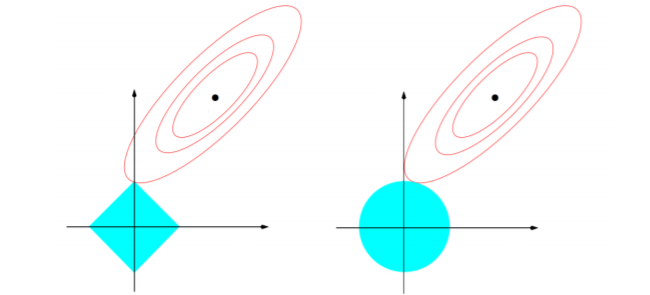
\includegraphics[width=.6\textwidth]{figures/lasso_v_ridge.png}
	\caption{Lasso on left, ridge on right; lasso prefers solutions along coordinate axes (i.e. sparse)}
\end{figure}

If we incorporate an offset,
%
\begin{align}
	\hat{w},\hat{b} &= \argmin_{w,b} \sum_{i=1}^n \left(y_i - (x_i^T w + b)\right)^2 + \lambda \|w\|_1,
\end{align}
%
but joint optimization is a pain, so let's prefer to de-mean our data. This is still actually kind of tricky minimization; the 1-norm isn't differentiable at the origin and this complicates things. Do by coordinate descent, minimize one direction at a time. This is guaranteed to approach the optimum for lasso (which is nice), but how do we pick our order of coordinate descent? Options,
%
\begin{itemize}
	\item Random each time
	\item Round robin
	\item Try to pick ``important'' coordinates (biases us).
\end{itemize}

Let's see an example. Take $j \in \{1,\ldots,d\}$.
%
\begin{align}
	\sum_{i=1}^n \left(y_i - x_i^T w\right)^2 + \lambda \|w\|_1 &= \sum_{i=1}^n \left(y_i - \sum_{k=1}^d x_{i,k} w_k\right)^2 + \lambda \sum_{k=1}^d |w_k|\\
	&= \sum_{i=1}^n \left(\left(y_i- \sum_{k\neq j} x_{i,k} w_k \right) - x_{i,j} w_j \right)^2 + \lambda \sum_{k\neq j} |w_k| + \lambda |w_j|.
\end{align}
%
So set $\hat{w}_k = 0$ for $k \in \{1,\ldots,d\}$ and loop over points:
%
\begin{align}
	r_i^{(j)} &= \sum_{k\neq j} x_{i,j} \hat{w}_k\\
	\hat{w}_j &= \argmin_{w_j} \sum_{i=1}^n \left(r_i^{(j)} - x_{i,j} w_j \right)^2 + \lambda |w_j|.
\end{align}

Pulling out one 1-d problem at a time! Works b/c lasso objective is \emph{separable}. Except\ldots this isn't actually a lot better. Hard to optimize because of pointy bit. Need to extend some concept of derivative and convexity. Traditional definition for fn is that lines b/t points on $f(x)$ lie above $f(x)$ (epigraph is convex). We need a different one here:
%
\begin{align}
	f(y) &\geq f(x) + \nabla f(x)^T (y-x) \quad \forall x,y
\end{align}
%
This amounts to saying that there's a ``supporting hyperplane'' touching the epigraph at $x$ such that the epigraph lies entirely on one side of the plane. If the function is differentiable at $x$, this is going to be the tangent plane. If not, we may have \emph{many} options, and these are called \emph{subgradients} (denoted $\partial_{w_j}$ for subgradient set at $w_j$). We call differentiable functions extremized at $x$ where $\nabla f(x) = 0$, and similarly we will call other functions extremized when $f(x)$ admits 0 as a subgradient at $x$.

OK, so how do we actually take subgradients and set them to zero? Consider example,
%
\begin{align}
	\partial_{w_j} \left(\sum_{i=1}\left(r_i^{(j)} - x_{i,j} w_j\right)^2 + \lambda |w_j|\right) &= \left\{\begin{array}{lr}
		a_j w_j - c_j - \lambda & \text{if } w_j < 0\\
		\left[-c_j - \lambda, -c_j + \lambda\right] & \text{if } w_j = 0\\
		a_j w_j - c_j + \lambda & \text{if } w_j > 0\\
		\end{array}\right.,
\end{align}
%
where
%
\begin{align}
	a_j &= \left(\sum_{i=1}^n x_{i,j}^2\right), &
	c_j &= 2\left(\sum_{i=1}^n r_i^{(j)} x_{i,j}\right).
\end{align}
%
This tells us how to do our minimization (look for regime that contains zero as subgrad):
%
\begin{align}
	\hat{w}_j &= \left\{\begin{array}{lr}
		\frac{c_j + \lambda}{a_j} & \text{if } c_j < -\lambda\\
		0 & \text{if } |c_j|\leq \lambda\\
		\frac{c_j - \lambda}{a_j} & \text{if } c_j > \lambda\\
		\end{array}\right.
\end{align}
%
where, recall,
%
\begin{align}
	a_j &= \sum_{i=1}^n x_{i,j}^2 & c_j &= 2 \sum_{i=1}^n \left(y_i - \sum_{k\neq j} x_{i,k} w_k\right) x_{i,j}.
\end{align}
%
This central flattening behavior provides ``soft thresholding''; can make predictor entries identically zero depending on strength of regularization.






















\section{Classification problems}
Different from regression! Same principles though. Need a loss function; what is? Let's start with binary classification, want to learn $f: X \to Y$ where $X$ contains features, $Y \in \{0,1\}$ is target class. Natural loss is 0/1 function: $\bm{1} \{f(X) \neq Y \}$. Expected loss is then
%
\begin{align}
	\mathbb{E}_{XY} \left[\bm{1}\{f(X) \neq Y\}\right] &= \mathbb{E}_X \left[\mathbb{E}_{Y\mid X}\left[\bm{1}\{f(x) \neq Y\} \mid X=x\right]\right]\\
	&= \mathbb{E}_X \bigg\{ \bm{1}\{f(x)=1\}\mathbb{P}(Y=0 \mid X=x) + \bm{1}\{f(x)=0\}\mathbb{P}(Y=1 \mid X=x) \bigg\}.
\end{align}
%
Supposing we know $P(Y\mid X)$, the Bayes optimal classifier is 
%
\begin{align}
	f(x) &= \argmax_{y} \mathbb{P}(Y=y \mid X=x).
\end{align}

How do we actually estimate $\mathbb{P}(Y \mid X)$? Well, can't do linear, and we're out of tricks now. Need a new trick; some function that goes from $\mathbb{R}^d$ to $[0,1]$ (called link function). A nice option is the sigmoid/logistic curve:
%
\begin{align}
	\mathbb{P}(Y=0 \mid X,W) &= \frac{1}{1+\exp\left[w_0 + \sum_i w_i X_i\right]}.
\end{align}
%
Still a sort of linear model in terms of what we do to our data variables. Note that $w_0$ applies a horizontal shift, and the $w_i$ ``stretch'' the curve. Note a nice property for binary classification, which is that
%
\begin{align}
	\frac{\mathbb{P}(Y=1 \mid w,X)}{\mathbb{P}(Y=0 \mid w,X)} &= \exp\left[w_0 + w^T X\right].
\end{align}
%
Reasonable to make our rule to classify as 1 if ratio is greater than 1, classify as 0 if ratio is less than 1. Equivalent result,
%
\begin{align}
	\ln \frac{\mathbb{P}(Y=1 \mid w,X)}{\mathbb{P}(Y=0 \mid w,X)}  = w_0 + \sum_i w_i X_i \to \left\{
		\begin{array}{l}
			< 0 \implies \text{ classify as 0}\\
			> 0 \implies \text{ classify as 1}\\
		\end{array}\right..
\end{align}

Alternative formulation (conditional likelihood): say $y \in \{-1,1\}$ instead of $\{0,1\}$ so we can then write
%
\begin{align}
	\mathbb{P}(Y=y \mid x,w) &= \frac{1}{1+\exp\left(-y w^T x\right)}
\end{align}
%
and find the MLE:
%
\begin{align}
	\hat{w}_\mathrm{MLE} &= \argmax_w \prod_{i=1}^n \mathbb{P}(y_i \mid x_i,w)\\
	\hat{w}_\mathrm{MLE} &= \argmin_w \sum_{i=1}^n \underbrace{\log\left(1+ \exp\left(-y_i x_i^T w\right) \right)}_{\sigma(y_i x_i^T w)}
\end{align}
%
Call the objective $J(w)$ (logistic loss): what the hell does it look like? Is it convex? (Yes.) How do we minimize it? Note that for an argument $z$, $\sigma(z) \sim |z|$ as $z \to -\infty$ and $\sigma(z) \to 0$ as $z \to +\infty$. In between, does some nonsense. So $\sigma(z)$ is easy to understand, but what about $J(w)$? Generally, no closed form in terms of $w$, can't just take derivative and set to zero. It turns out, moreover, that if we happen to have a $w$ that correctly classifies every point (by dumb luck; linearly separable data set), then $y_i x_i^T w$ is strictly positive and so for $t > 0$, $y_i x_i^T (tw) > y_i x_i^T w$ and we will always prefer to infinitely extend our $w$ along our ``good'' direction to continue reducing loss. This breaks the classifier. Sigmoid classifiers become step functions. We \emph{need} to regularize this conditional log likelihood objective.













\section{Interlude: Gradient descent}
Recall that our general problem is to be handed i.i.d. data $\{(x_i,y_i)\}_{i=1}^n$ with $x_i \in \mathbb{R}^d$ and $y_i \in \mathbb{R}$, a model with some parameters $w$, and some loss function depending on $w$ to be calculated on our data, then optimize $w$ with respect to that loss. The computational meat is in optimization. We turn it into a problem that looks like $X^T X w = X^T Y$, but how do we actually do that? Lots of different ways! Many algorithms! Some depend on properties of matrices, sparseness, etc. Let's look at one in particular, which is gradient descent.

Say I have some function $f(x)$ where $x \in \mathbb{R}^d$. Taylor tells us that
%
\begin{align}
	f(x + \delta) &= f(x) + \nabla f(x) \cdot \delta + \cdots,
\end{align}
%
so at any point we can find the gradient and take a step in the opposite direction, which must decrease $f$. Ex:
%
\begin{align}
	f(w) &= \frac{1}{2} \|X w - y\|_2^2\\
	\nabla f(w) &= X^T(Xw -y) = X^T (Xw -y) = X^T X w - X^T y,
\end{align}
%
so if we are at some $w_t$ our next step should be
%
\begin{align}
	w_{t+1} &= w_t - \eta X^T(X w_t - y).
\end{align}
%
Examine recursion behavior, find (for optimum $w_\ast$) that
%
\begin{align}
	(w_{t+1} - w_\ast) &= \left(I - \eta X^T X \right)^{t+1} (w_0 - w_\ast),
\end{align}
%
so can bound rate of approach to optimum. (Shocker: need $\eta$ small.)


We can do one better by going one step further down the Taylor series,
%
\begin{align}
	f(y) &\approx f(x) + f'(x) (y-x) + \frac{1}{2} f''(x) (y-x)^2
\end{align}
%
make our next step the minimum
%
\begin{align}
	\tilde{y} &= \frac{f'(x)}{f''(x)}
\end{align}










\section{Perceptron}
Recall binary classification: we want to learn $f: X \to Y$ with loss $\ell(f(x),y) = \bm{1}\{f(x)\neq y\}$. Expected loss
%
\begin{align}
	\mathbb{E}_{XY} \left[\bm{1}\{f(X)\neq Y\}\right] &= \mathbb{E}_X\left[\mathbb{E}_{Y\mid X} \left[\bm{1}\{f(x) \neq Y\}\mid X=x\right]\right]\\
	\mathbb{E}_{Y\mid X} \left[\bm{1}\{f(x) \neq Y\}\mid X=x\right] &= 1 - P\left(Y=f(x) \mod X=x\right),
\end{align}
%
so obviously want Bayes classifier
%
\begin{align}
	f(x) &= \argmax_{y} \mathbb{P}\left(Y=y\mid X=x\right),
\end{align}
%
and often take a logistic model like
%
\begin{align}
	P(Y=y\mid x,w) &= \frac{1}{1+ \exp(-yw^T x)}.
\end{align}
%
Buuuuuut it's really hard to know if that model's good. Often probably isn't. Can we do this without a model? Certainly it's not hard to do it with our eyeballs. Can we give our computer eyeballs? Yup!

Say we're classifying to $y \in \{-1,1\}$ and take a linear model where we predict $\sgn(w^T x + b)$. Start with $w_0 = 0, b_0 = 0$, get a data point $x_k$, predict $y_k$, check, and if we were wrong, update
%
\begin{align}
	\begin{bmatrix}w_{k+1}\\b_{k+1}\\\end{bmatrix} &= \begin{bmatrix}w_k\\b_k\\\end{bmatrix} + y_k \begin{bmatrix}x_k\\1\\\end{bmatrix}.
\end{align}
%
Basically we rotate/shift our classification line until we get everything right. Guaranteed to converge if we have linearly separable data! If $\gamma$ is the width of the widest margin (hyperplanar slab separating classes) and feature vector norms are bounded by $\|x_k\| \leq R$, then there is a theorem (Block, Novikoff): if we have a sequence of examples $(x_t,y_t)$, then the number of mistakes made by the perceptron is bounded by $R^2 / \gamma^2$ for \emph{any} such sequence. Convergence is guaranteed and \emph{fast}.

This is pretty dank, but\ldots we can't really do much with it. Most things aren't linearly separable (or even separable at all!), and even a single point in the way of separability can cause infinite cycling and destroy convergence. So why do we care at all? Well, it's a totally different way of thinking about learning! Previously we wrote down a model and then developed an algorithm that optimizes it. Here we did exactly the opposite: wrote down an algorithm and analyzed it. Is there an equivalent modeling problem? What is the perceptron optimizing? Does it have a definable loss function? This all leads to support vector machines (SVMs).

















\section{Support vector machines}
The perceptron model admitted many possible classifiers for a given data set, and it liked them all just as well, but we are not so generous. Some seem to skirt very close to the edges of our classes, which feels dangerous, and we'd be more comfortable with a boundary as far from our known data as possible, considering that our data may suffer perturbations on future collections.

How can we pick the ``safest'' classifier? Consider some hyperplane boundary $x^T w + b = 0$ that we've trained, and the closest point $x_0$ to it. How close is it? Let
%
\begin{align}
	\tilde{x}_0 &= \argmin_{z \in \{x : x^T w + b = 0\}} \|z - x_0 \|_2^2
\end{align}
%
be the closest point on the hyperplane to $x_0$. Then
%
\begin{align}
	\|x_0 - \tilde{x}_0\|_2 &= \left\|\frac{w^T}{\|w\|_2} (x_0-\tilde{x}_0)\right\|,
\end{align}
%
but we know that $w^T \tilde{x}_0 = -b$, so
%
\begin{align}
	\|x_0 - \tilde{x}_0\|_2 &= \frac{|w^T x_0 + b|}{\|w\|_2}.
\end{align}
%
So if we now call $\gamma$ the distance from the classification boundary to a parallel hyperplane on either side, our problem is to maximize $\gamma$ over $w$ and $b$ subject to
%
\begin{align}
	\frac{y_i(x_i^T w + b)}{\|w\|_2} &\geq \gamma \qquad \forall i
\end{align}
%
where the sign $y_i$ makes sure we're paying attention to points on both sides of the boundary correctly. This problem ends up being equivalent, however, to the minimization of $\|w\|_2^2$ subject to
%
\begin{align}
	y_i\left(x_i^T w + b\right) & \geq 1 \qquad \forall i,
\end{align}
%
which gives us both our optimal hyperplane and a measure of our separability for free.




However, this still breaks for non-separable data! To make this useful, we need to permit some misclassification or a smaller margin! We implement this as minimizing $w$ subject to
%
\begin{align}
	y_i(x_i^T w + b) &\geq 1 -\xi_i\\
	\xi_i &\geq 0\\
	\sum_j \xi_j &< \nu.
\end{align}
%
We now have a knob to trade off between $\nu$ and $\|w\|_2$. The $\xi_i$ are called support vectors (samples on the margin).

Constrained optimization sucks, but as we found with lasso, we have some tricks. Specifically, for any $\nu \geq 0$, there is a $\lambda \geq 0$ such that we can just as well minimize
%
\begin{align}
	\sum_{i=1}^n \max\{0, 1 - y_i(b + x_i^T w)\} + \lambda \|w\|_2^2.
\end{align}

We're back in machine learning land, now! We have a loss function
%
\begin{align}
	\ell_i(w) &= \max\{0, 1 - y_i x_i^T w\}
\end{align}
%
which we call the \emph{hinge loss} and can optimize by any of the methods we've talked about before. Fact: this is exactly the loss being optimized by the perceptron!
%
\begin{align}
	\nabla_w \ell_i(w,b) &= \left\{
	\begin{array}{ll}
		-y_i x_i + \frac{2\lambda}{n} w & \text{if } 1-y_i(b+x^T w) > 0\\
		\frac{2\lambda}{n} w & \text{otherwise}\\
	\end{array}\right.	
\end{align}
%
SGD update for this objective is the perceptron with the right parameters! (The kink in hinge loss is what gives us the ``give up'' behavior in perceptron?) Note that Newton's method does not work on hinge loss, but it has subgradients so SGD still works.


Note that logistic regression assumed a data model $\mathbb{P}(Y=y \mid X=x, w)$ that's pretty rigid. It gives us confidence measurements, but how confident are we in our confidence? SVM doesn't force us to assume such a model, so can we extract confidence that we trust from that? Yes! Our SVM predictor gives us a bunch of predictions $y_i = \sgn(w^T x_i)$. Isotonic regression is the fitting of a function to that data that interpolates those predictions (possibly logistic).






\section{Bootstrap}
So cross-validation was pretty good technology, but it has downsides, for example throwing out a fifth of our data. The validation error was useful, but the only real statistical power was for constraining the mean via Hoeffding's inequality, which doesn't help with other statistical figures. Further, we get errors for the population, but not really for individual data points. Enter the bootstrap black magicks.

Say we have a dataset $\mathcal{D} = \{z_1,\ldots,z_n\}$ drawn i.i.d from some CDF $F_Z$. We want to compute a statistic $\hat{\theta} = t(\mathcal{D})$ (say the variance). We can calculate the empirical CDF
%
\begin{align}
	\hat{F}_{n,Z}(x) &= \frac{1}{n} \sum_{i=1}^n \bm{1}\left\{z_i \leq x\right\}
\end{align}
%
and we know that $\mathbb{E}\left[\hat{F}_{n,Z}(x)\right] = F_Z(x)$. Say I could get more data: $\{\mathcal{D}_1,\mathcal{D}_2,\ldots,\mathcal{D}_b\}$ from the same distribution. Then I can get a distribution of $\hat{\theta}_i = t(\mathcal{D}_i)$ and can compute stats on stats on stats!

But it's hard to get a bunch of data sets, often! Fortunately we have an estimate of $F_Z(x)$ lying around, which is to say $\hat{F}_{n,Z}(x)$; why not draw our new data sets from that? We know that it will converge toward the true CDF for large $n$. So let's generate $\mathcal{D}^{\ast b} = \{z_1^{\ast b}, \ldots, z_n^{\ast b}\}$ drawn from $\hat{F}_{n,Z}$ with replacement and get $\theta^{\ast b} = t(\mathcal{D}^{\ast b})$ then compute statistics on these $\theta^{\ast b}$, which should be good estimates of the true statistics.


What do we do with this? Whatever we want! We can fit a function to some data, then fit 1000 more with bootstrap and get a confidence interval for \emph{every single point}. This is crazy. Caveat: need lots of data. It has powerful asymptotic guarantees, but they don't really become good constraints until big $n$ and it's hard to tell how big is big enough. Further, this can involve a lot of computation if you want tight bounds, and there are statistics that it does not work well for.











\section{Decision theory; discriminative vs. generative learning}
Recall in binary classification, we talked about classifying according to
%
\begin{align}
	f(x) &= \argmax_y \mathbb{P}(Y=y \mid X=x),
\end{align}
%
but it's totally equivalent according to Bayes to look at
%
\begin{align}
	f(x) &= \argmax_y \mathbb{P}(X=x \mid Y=y) \mathbb{P}(Y=y),
\end{align}
%
where we think about the distribution of features given a certain outcome. Need to scale based on probability of outcome to predict!


Consider an example where
%
\begin{align}
	\mathbb{P}(X=x) &\equiv (1-\pi) P_0(x) + \pi P_1(x)
\end{align}
%
where $0\leq\pi \leq 1$ and $P_0(x) = \mathcal{N}(x; \mu_0, \sigma^2)$ and $P_1(x) \mathcal{N}(x;\mu_1,\sigma^2)$. The Bayes classifier is
%
\begin{align}
	f(x) = 1 \text{ if } \frac{P_1(x) \pi}{P_0(x) (1-\pi)} \geq 1.
\end{align}
%
This comes out to
%
\begin{align}
	f(x) = 1 \text{ if } x \geq \frac{\mu_1 +\mu_0}{2} - \frac{\sigma^2}{\mu_1 - \mu_0} \log\left(\frac{\pi}{1-\pi}\right).
\end{align}
%
Can see that as $\pi$ grows, decision boundary shifts left, and vice-versa.

This generalizes to more dimensions! If we have Gaussian feature distributions for each class with the same covariance, we will get a hyperplane classification boundary (linear discriminant analysis). If they have different covariances, quadratic boundary (quadratic discriminant analysis).

Say we measure $\{(x_i,y_i)\}_{i=1^n}$, then we get estimates
%
\begin{align}
	\hat{mu}_k &= \frac{1}{|\{i : y_i = k\}} \sum_{i:y_i=k} x_i\\
	\hat{Sigma}_k &= \frac{1}{|\{i:y_i = k\}|-1} \sum_{i:y_i = k} (x_i - \hat{\mu}_k)(x_i - \hat{\mu}_k)^T.
\end{align}

So discriminative learning directly attempts to model $\mathbb{P}(Y=y \mid X=x)$ (e.g. SVM, logistic classification), while generative learning goes after $\mathbb{P}(X=x,Y=y) = \mathbb{P}(X=x\mid Y=y) \mathbb{P}(Y=y)$. Is this more work? Yes! But often domain knowledge allows us to do some educated preparation.













\section{Hypothesis testing}
This is\ldots obviously important.

Say that we want to detect anomalous transactions in a credit log. For each transaction we observe some features $X$, and the transaction is either genuine ($Y=0$) or fraudulent ($Y=1$). In the first case $H_0$, $X$ is drawn from a distribution $P_0$ for genuine transactions, and in $H_1$ it is drawn from $P_1$. We want to determine which population our feature vector is drawn from by some (possibly randomized) decision function $\delta(X)$.

In Bayesian hypothesis testing, we assume priors $\mathbb{P}(Y=1) = \pi$ and $\mathbb{P}(Y=0) = (1-\pi)$ and want to minimize $\mathbb{P}_{XY}(Y \neq \delta(X))$. (It turns out that there will always be deterministic dudes that live in this set.) Effectively this is weighting distributions for decision according to priors.


We can retune our priorities by instead looking for
%
\begin{align}
	\argmin_\delta \max\{\mathbb{P}(\delta(X) = 0\mid Y=1), \mathbb{P}(\delta(X) =1 \mid Y=0)\},
\end{align}
%
which is known as minimax hypothesis testing.



There is also Neyman--Pearson hypothesis testing where we choose
%
\begin{align}
	\argmax_\delta \mathbb{P}(\delta(X) = 1 \mid Y=1) \text{ subject to } \mathbb{P}(\delta(X)=1\mid Y=0) \leq \alpha.
\end{align}
%
This maximizes true positives subject to a bounded false alarm rate $\alpha$. The wacky thing is that there is always an optimal test $\delta^\ast$ following
%
\begin{align}
	\mathbb{P}(\delta^\ast(X) =1) &= \left\{\begin{array}{lr}
		1 & \text{ if } \frac{P_1(x)}{P_0(x)} > \eta\\
		\gamma & \text{ if } \frac{P_1(x)}{P_0(x)} = \eta\\
		0 & \text{ if } \frac{P_1(x)}{P_0(x)} < \eta
	\end{array}\right..
\end{align}
%
such that the false alarm rate is \emph{exactly} $\alpha$.

All hypothesis tests are effectively a trade-off between false alarm rate and detection power. Different algorithms will have different trade-off curves (ROC curves), and we can assess them on this basis.














\subsection{p-values}
We are often confronted with problems where we (hopefully) have a strong model for the null hypothesis distribution, but no real model for non-null hypotheses (e.g. real vs. fraudulent purchases, since fraud is often strategic/adaptive). Can we test here? Yuuuup.



One definition is that the p-value is the probability of finding data at least as extreme if the null hypothesis is true (that is, $X \sim P_0$). Alternatively, the p-value is a uniform r.v. derived from $X$ in the case that $X \sim P_0$. (And note: \emph{any} such uniform variable. There are many possible definitions!) This second rule will do us more favors. The first might lead us to suspect that a particular $H_1$ is true, and that's very bad.

Say that we have $P_0(x) = \mathcal{N}(x;\mu_0, \sigma^2)$ and observe $x_i \in \mathbb{R}$. The p-value is
%
\begin{align}
	p_i &= P_0(X \geq x_i)\\
	    &= \int_{x=x_i}^\infty \frac{1}{\sqrt{2\pi\sigma^2}} e^{-\frac{(x-\mu_0)^2}{2\sigma^2}} \d x\\
	    &= 1 - F\left(\frac{x_i-\mu_0}{\sigma}\right).
\end{align}
%
The correct way to use this information is to pick a threshold (e.g. $\alpha = 0.05$), measure data $x_i$, then calculate $p_i$ (uniform on $[0,1]$ under $H_0$). Then the test is that if $p_i \leq \alpha$, we reject $H_0$. (Or, more generally, we can define any weird rejection region we want, as long as it has measure no greater than $\alpha$.)


Note that the uniformity of $p$ under $H_0$ presents a danger: repeated measurements can easily land us in the rejection region by chance! Say we measure $x_i \sim \mathcal{N}(\mu,1)$ each day $i$ and take $H_0: \mu=0$. We can define a running average
%
\begin{align}
	Z_i &= \frac{1}{\sqrt{i}} \sum_{j=1}^i x_j
\end{align}
%
and under $H_0$ we have $Z_i \sim \mathcal{N}(0,1)$ so that we can define a $p$-value
%
\begin{align}
	p_i &= \frac{1}{2\pi} \int_{z=z_i}^\infty e^{-\frac{z^2}{2}} \d z.
\end{align}
%
The danger is that \emph{eventually} we will measure some $p_i \leq \alpha$. If we declare victory here, our stopping time was not independent of our measurements; it is much like tainting our learning process by touching the test data. Caution!










\subsection{Multiple testing}
Take a genetics example: 13,071 drosophila genes potentially affecting virus replication. Knock out one gene at a time, infect microwell array, count fluorescent signals distributed $x_i \sim \mathcal{N}(\mu_i,1)$ (not actually, but play along).

For each gene $i$, we have a null hypothesis $H_0(i) : \mu_i = 0$, i.e. it plays no role in virus inhibition. Procedure:
%
\begin{description}
	\item[Set:] $\alpha=0.05$
	\item[Observe:] $x_i \in \mathbb{R}$
	\item[p-value:] $p_i = P_0(X \geq x_i)$
	\item[Test:] If $p_i \leq \alpha$, reject $H_0(i)$
\end{description}

How many genes do we expect to meet the rejection criterion under $H_0$? If $I_0$ is the set of $i$ for which $H_0(i)$ is true,
%
\begin{align}
	\mathbb{E}\left[\sum_{i\in I_0} \bm{1}\{p_i \leq \alpha\}\right] &= \sum_{i \in \mathbb{I}_0} \mathbb{P}(p_i \leq \alpha) = |I_0| \alpha.
\end{align}
%
This is an\ldots alarming rate of false alarms. We can measure this badness by the family-wise error rate (FWER) which is the probability of rejecting any true null. If we adopt the Bonferroni rule (reject $i$ if $p_i \leq \alpha/n$), then
%
\begin{align}
	\mathrm{FWER} &= \mathbb{P}\left(\bigcup_{I_0} \{p_i \leq \frac{\alpha}{n}\}\right)\\
	&= \leq \sum_{i \in I_0} \mathbb{P}\left(p_i \leq \frac{\alpha}{n}\right)
	&= \sum_{i \in I_0} \frac{}{}
\end{align}




This might be a little harsh. Perhaps better to judge by false discovery rate (FDR); we can tolerate a few errors if we get enough true discoveries.
%
\begin{align}
	\mathrm{FDR} &\equiv \mathbb{E}\left[\frac{|I_0 \cap R|}{|R|}\right]
\end{align}
%
where $R$ is the rejection set. There is a procedure called the Benjamini--Hochberg procedure:
%
\begin{itemize}
	\item Sort p-values so that $p_{(1)} \leq p_{(2)} \leq \cdots \leq p_{(n)}$
	\item $i_\mathrm{max} = \max\left\{i : p_{(i)} \leq \frac{i}{n} \alpha\right\}$
	\item $R = \{i: i \leq i_\mathrm{max}\}$
\end{itemize}
%
where $R$ is our rejection set. A theorem tells us that $BH(\alpha)$ satisfies $\mathrm{FDR} \leq \alpha$.
















\section{Bayesian methods}
Everything we've just been over is pretty classical, nothing really new after 1900. Let's move on a bit. Recall our MLE example about determining the weighting $\theta$ of a coin. Suppose we were told that based on past knowledge the coin is around 50--50, so we have some \emph{prior belief} $P(\theta)$. Bayes sez
%
\begin{align}
	P(\theta \mid \mathcal{D}) &= \frac{P(\mathcal{D}\mid \theta) P(\theta)}{P(\mathcal{D})}.
\end{align}
%
The likelihood function, we know, is the binomial
%
\begin{align}
	P(\mathcal{D} \mid \theta) &= \theta^{\alpha_H} (1- \theta)^{\alpha_T},
\end{align}
%
where $\alpha_H, \alpha_T$ are our drawn data. There are many options for prior distribution, but some (conjugate priors) are more natural, and for a binomial likelihood we want to take
%
\begin{align}
	P(\theta) &= \frac{\theta^{\beta_H - 1} (1-\theta)^{\beta_T-1}}{B(\beta_H,\beta_T)} \sim \mathrm{Beta}(\beta_H,\beta_T),
\end{align}
%
can be shown to have
%
\begin{align}
	\mathrm{mean} &= \frac{\beta_H}{\beta_H + \beta_T}\\
	\mathrm{mode} &= \frac{\beta_H - 1}{\beta_H + \beta_T - 2},
\end{align}
%
while variance is narsty. Very tunable distribution. It is convenient (conjugate) because when we have a binomial likelihood and beta prior, the posterior distribution will \emph{also} be beta! 
%
\begin{align}
	P(\theta\mid \mathcal{D}) &\propto \theta^{k+\beta_H-1} (1-\theta)^{n-k+\beta_T-1} = \mathrm{Beta}(k+\beta_H, n-k+\beta_T)
\end{align}
%
if we measured $k$ heads and $(n-k)$ tails. We just update parameters according to data! We now have an inference rule: update our posterior, then make estimates like
%
\begin{align}
	\mathbb{E}[\theta] &= \int_0^1 \theta P(\theta\mid\mathcal{D}) \d \theta\\
	\mathbb{E}[f(\theta)] &= \int_0^1 f(\theta) P(\theta\mid\mathcal{D}) \d \theta,
\end{align}
%
and more complicated statistics! We have a full distribution estimate based on data. This said, these integrals might be super difficult.

Alternative: maximum \emph{a posteriori} approximation (MAP)!
%
\begin{align}
	\hat{\theta}_{\mathrm{MAP}} &= \argmax_\theta P(\theta \mid \mathcal{D})\\
	\mathbb{E}[f(\theta)] &\approx f(\hat{\theta}).
\end{align}
%
In the coin-flip example,
%
\begin{align}
	\hat{\theta} &= \frac{k + \beta_H - 1}{n - k + \beta_T - 1}.
\end{align}




Let's take a moment to think about the foundational differences between frequentist stats (which we've been doing) and Bayesian (which we're doing now). In the frequentist perspective, we treat $\theta$ as a fixed hidden parameter to be estimated, and the data we draw as random and controlled by $\theta$. However, Bayesians would say that our data is our data is \emph{the} and we should not expect that there is some ``true'' model out there with fixed parameters. Instead, we should think about the distribution of $\theta$ compatible with the data observed. (There are some flame wars.)
























\section{Nearest neighbor}
Say we have some gnarly decision problem. The Bayes decision boundary may be real jacked up. How do we capture that? We only know about linear decision boundaries with various degrees of flexibility (e.g. SVM). Very low variance, but ridiculous bias. Usually wrong for any interesting boundary.

Let's go to the other end: nearest neighbor classification. Take a point in the domain, look at the $n$ (say 15? 1? 600?) nearest data points and ask them for a majority vote. Whoever wins, wins the point. Repeat until satisfied. Smaller number of neighbors makes very fragmented boundary, hard to trust. Great training error (``you're just classifying yourself''), but abysmal test error. Too many neighbors makes both pretty bad. We also have several choices for what we mean by distance.

If we draw some $\{(x_i,y_i)\}_{i=1}^n \subset \mathbb{R}^d \times \{1,\ldots,k\}$ and assume that as $n \to \infty$ the $x_i$ become dense in $\mathbb{R}^d$ and that $\mathbb{P}(Y=j\mid X=x)$ is smooth, then it is guaranteed that the 1-NN error rate is
%
\begin{align}
	\mathbb{P}(Y_a \neq Y_b) &= \sum_{\ell=1}^k \mathbb{P}(Y_a = \ell, Y_b \neq \ell) = \sum_{\ell=1}^k p_\ell(1-p_\ell) \leq 2 (1-p_{\ell^\ast}) - \frac{k}{k-1} (1-p_{\ell^\ast})^2,
\end{align}
%
which in the last step we see is bounded by twice the Bayes error. This is cool!

Unfortunately, the density assumption is crippling. In high dimension, the expected distance to the nearest neighbor stays pretty big even for big data. It's likely for all of our data to be in the ``corners'' of the domain; everything is far from everything. This is scary for local methods, called the ``curse of dimensionality.''

Still, in low dimension it's perfectly fine, and we can of course do regression with this, too; just average up nearby points and predict the middle. Can improve by weighting average according to some smoothing kernel, or doing local linear regression. All v. effective in low dimension, though potentially computationally expensive: it's hard to \emph{find} nearest neighbors in the first place!



















\section{Kernel hijinks}
Sometimes we may be confronted with things that are not linearly separable. What do? Well, we can always map into more dimensions until they \emph{are} separable. One nice way is polynomial feature maps $\phi(x) : \mathbb{R}^d \to \mathbb{R}^p$. We can encode these maps as vectors of all monomials of a given degree: if we have a data point $u \in \mathbb{R}^2$, for example, we can define
%
\begin{align}
	\begin{array}{lrr}
	d = 1:& \phi(u) =& \begin{bmatrix}u_1\\u_2\\\end{bmatrix}\\
	d = 2:& \phi(u) =& \begin{bmatrix}u_1^2\\u_2^2\\u_1u_2\\u_2u_1\\\end{bmatrix}\\
	\vdots &&\\
	\text{general }d :& \dim(\phi(u)) \sim& p^d \text{ for } u\in \mathbb{R}^p.\\
	\end{array}
\end{align}
%
Can generate arbitrary multivariate polynomials in $u_i$ and $v_i$ via dot product between $\phi(u)$ and $\phi(v)$.

Great, we can make huge polynomials. Why do we care? Kernel trick! Say we have
%
\begin{align}
	\hat{w} &= \argmin_{w} \sum_{i=1}^n \left(y_i - x_i^T w\right)^2 + \lambda \|w\|_w^2.
\end{align}
%
A theorem says that there exists $\alpha \in \mathbb{R}^n$ such that
%
\begin{align}
	\hat{w} &= \sum_{i=1}^n \alpha_i x_i
\end{align}
%
(where recall, $x_i \in \mathbb{R}^d$). What is this $\alpha$?
%
\begin{align}
	\hat{\alpha} &= \argmin_{\alpha} \sum_{i=1}^n \left(y_i - \sum_{j=1}^n \alpha_j \braket{x_j,x_i}\right)^2 + \lambda \sum_{i,j=1}^n \alpha_i \alpha_j \braket{x_i,x_j}\\
	\hat{\alpha} &= \argmin_{\alpha} \sum_{i=1}^n \left(y_I - \sum_{j=1}^n \alpha_j K(x_i,x_j)\right)^2 + \lambda \sum_{i,j=1}^n \alpha_i \alpha_j K(x_i,x_j)\\
	\hat{\alpha} &= \argmin_\alpha \|y - K\alpha\|_2^2 + \lambda \alpha^T K \alpha,
\end{align}
%
where
%
\begin{align}
	K_{ij} = K(x_i,x_j) \equiv \braket{\phi(x_i),\phi(x_j)}.
\end{align}
%
For $\lambda$ large enough to make $K+\lambda I$ p.d., we have
%
\begin{align}
	\hat{\alpha} (K+\lambda I)^{-1} y.
\end{align}
%
In practice, $K$ is often already p.d., so why do we regularize? Without it, we will trivially overfit any dataset, since we get $n$ dof to work with.

The magic is that $\phi$ above doesn't actually have to be a polynomial map. It can map to \emph{any} inner-product space and the optimization procedure will go through fine. We don't even have to know what $\phi$ or the target space actually is as long as the kernel function $K(x,x')$ satisfies Mercer's condition: $K_{ij} = K(x_i,x_j)$ is PSD for any pointset $\{x_1,\ldots,x_n\}$.


Some common kernels:
%
\begin{itemize}
	\item Degree d polys --- $K(u,v) = (u \cdot v)^d$
	\item Degree $\leq d$ polys --- $K(u,v) = (u\cdot v + 1)^d$
	\item Gaussian --- $K(u,v) = \exp\left[-\frac{\|u-v\|_2^2}{2\sigma^2}\right]$
	\item Sigmoid --- $K(u,v) = \tanh(\eta u\cdot v + \nu)$
\end{itemize}

The Gaussian (also called RBF) kernel is especially useful. Essentially weights by bumps centered around data points, but now we're training for the weight of each point, and have some hyperparameters to tune ($\lambda$ and $\sigma$).

This was actually what we did with those weird random features in MNIST ridge regression. We used
%
\begin{align}
	\phi(x) &= \begin{bmatrix}\sqrt{2}\cos(w_1^T x + b_1)\\\vdots\\\sqrt{2}\cos(w_p^T x + b_p)\\\end{bmatrix}
\end{align}
%
with $w_k \sim \mathcal{N}(0,2\gamma I)$, $b_k \sim \mathrm{uniform}(0,\pi)$. This was weird! The explicit map for the Gaussian kernel features is infinite-dimensional, and that's a hard matrix to store. What have we done? Look at the expected inner product of two points mapped with our random map:
%
\begin{align}
	\mathbb{E}\left[\frac{1}{p}\phi(x)^T \phi(y)\right] &= \frac{1}{p} \sum_{k=1}^p \mathbb{E}\left[2\cos(w_k^T x + b_k)\cos(w_k^T y + b_k)\right]\\
	\mathbb{E}\left[\frac{1}{p}\phi(x)^T \phi(y)\right] &= \mathbb{E}_{w,b} \left[2\cos(w^T x + b)\cos(w^T y + b)\right]\\
	\mathbb{E}\left[\frac{1}{p}\phi(x)^T \phi(y)\right] &= e^{-\gamma\|x-y\|_2^2}.
\end{align}
%
We made a \emph{truncated} feature map which approximates the true kernel we want in expectation! (And $p=24000$ is nicer than infinite features\ldots)





















\section{Principal component analysis}
Overall idea is low-dimensional representation of high-dimensional stuff. Given $x_1,\ldots,x_n \in \R^d$ we want to find some $\lambda_1,\ldots,\lambda_n \in \R^q$ with $q \ll d$ such that $x_i \sim \mu + V_q \lambda_i$ where $V_q^T V_q = I_q$. To be more precise, we want to find $\mu$, $V_q$, and $\{\lambda_i\}$ attaining
%
\begin{align}
	\min_{\mu,V_q,\{\lambda_i\}} \sum_{i=1}^n \|x_i - \mu - V_q\lambda_i\|_2^2.
\end{align}
%
If we fix $V_q$, we find
%
\begin{align}
	\mu = \bar{x} &= \frac{1}{n} \sum_{i=1}^n x_i\\
	\lambda &= V_q^T (x_i - \bar{x})
\end{align}
%
and so are left to determine
%
\begin{align}
	\min_{V_q} \sum_{i=1}^n \|(x_i-\bar{x}) - V_q V_q^T (x_i - \bar{x})\|_2^2.
\end{align}
%
If we recall
%
\begin{align}
	\Sigma &= \sum_{i=1}^n (x_i-\bar{x})(x_i-\bar{x})^T,
\end{align}
%
then we see that
%
\begin{align}
	\min_{V_q} \sum_{i=1}^n \|(x_i-\bar{x}) - V_q V_q^T (x_i-\bar{x})\|_2^2 &= \min_{V_q} \left[\tr \Sigma - \tr V_q^T \Sigma V_q\right].
\end{align}
%
By eigenvalue decomposition of $\Sigma$, we can find that this minimum is achieved if we make the columns of $V_q$ the eigenvectors of $\Sigma$ with the $q$ biggest corresponding eigenvalues. Essentially, we are picking out the directions with the most variance and projecting our data down into them for legibility.
%
\begin{align}
	(X - \bm{1}\bar{x}^T) V_q &= U_q S_q
\end{align}
%
where $U_q$ is orthogonal and $S_q$ is a weight matrix, essentially. Why can we do this? Singular value decomposition!


\begin{thm}[SVD]
	Let $A \in \R^{m\times n}$ with rank $r \leq \min\{m,n\}$. Then $A = USV^T$ where $S \in \R^{r\times r}$ is diagonal, $U^T U = I_m$ and $V^T V = I_n$.
\end{thm}

Why do we care? Well, for $v_i$ a column of $V$,
%
\begin{align}
	A^T A v_i &= (USV^T)^T(USV^T)v_i = V S U^T U S V^T v_i = V S^2 V^T v_i,
\end{align}
%
and since columns of $V$ are orthonormal,
%
\begin{align}
	A^T A v_i &= V S^2 e_i = S_{ii}^2 V e_i = S_{ii}^2 v_i,
\end{align}
%
so we see that $v_i$ is an eigenvector of $A^T A$ with positive eigenvalue $S_{ii}^2$. A similar calculation for a column $u_i$ of $U$ shows that such columns are eigenvectors of $A A^T$ also with eigenvalues $S_{ii}^2$. (Compute eigenvalues of $A A^T$ or $A^T A$, whichever is smaller.)

This is nice because the SVD of $JX = X - \bm{1}\bar{x}^T$ gives eigenvectors of $\Sigma$, and projection onto them is exactly PCA! In particular,
%
\begin{align}
	(JX)(JX)^T = J XX^T J \equiv J K J = U S^2 U^T.
\end{align}
%
Recall in the kernel interpretation we are embedding in a high-dimensional space and then effectively projecting back down onto new principal components.






\section{SVD tricks}
Recall ridge regression, where
%
\begin{align}
	\hat{y} &= X (X^T X + \lambda I)^{-1} X^T y.
\end{align}
%
Consider SVD of $X$ and see that
%
\begin{align}
	\hat{y} &= \sum_{i=1}^d u_i u_i^T \frac{s_i^2}{s_i^2 + \lambda} y_i.
\end{align}
%
Notice that the fraction is nearly zero for $s_i^2 \ll \lambda$ and nearly unity for $s_i^2 \gg \lambda$, which reflects ridge regression's preference for high-variance directions to spend its limited predictor magnitude on.


\begin{thm}[Johnson--Lindenstrauss]
	Let $\e > 0$ and set $q = 20 \e^{-2} \log(n)$. Assume that $A \in \R^{d \times q}$ has entries sampled iid from $\mathcal{N}(0,1/q)$. For any $z \in \R^d$, we have, with probability at least $1 - 2 \exp\left[(\e^2-\e^3)q/4\right]$ that
	%
	\begin{align}
		(1-\e)\|z\|^2 \leq \|A^T z\|^2 \leq (1+\e)\|z\|^2.
	\end{align}
\end{thm}

This is a crazy tight bound on the magnitude of projected vectors. Tells us that we don't really ever have high-d data; we can always project down to about $\log(n)$ dimensions with virtually no loss of information by this random projection. Further, this bound applies to \emph{every point}, not just an average representation error like in PCA.

Alternatively, there is also non-negative matrix decomposition, which is apparently good?











\section{Matrix completion}
We've been doing a lot of formal wankery, but there is also a practical organization to this exploration: what do we actually want to do with this stuff and what are the methods for applying it? We've started with linear methods, and explored methods for turning nonlinear problems into linear ones. There is more, though! Matrix completion.

What do we do about missing data? Recall that we were guaranteed by the SVD theorem that we could bust up a matrix $A$ as
%
\begin{align}
	A &= \sum_{k=1}^r u_k v_k^T s_k,
\end{align}
%
and we use that representation to describe the rank-1 approximation task: for $\sigma>0$ and unit vectors $x \in \R^m$, $y \in \R^n$, minimize
%
\begin{align}
	\|\sigma xy^T  - A\|_F^2 \sigma^2 + \tr(A^T A) - 2 \sigma x^T A y\\
	&= \sigma^2 + \left(\sum_{k=1}^r s_k^2\right) - 2 \sigma\left(\sum_{k=1}^r x^T u_k v_k^T y s_k\right).
\end{align}
%
The best we can do is to make $\sigma = s_1$: cancel as much of the positive term as possible. This generalizes, in fact: the best rank-$p$ approximation to a matrix will be the first $p$ elements of the $SVD$ of our matrix.



This gives us a tool for filling in incomplete data. We could do something like zero-filling, or mean-filling, but we can be more principled. Find a predictor
%
\begin{align}
	\argmin_{U\in\R^{m\times d}, V\in\R^{n\times d}} \sum_{(i,j,s)\in\mathcal{S}} \|(UV^T)_{i,j} - s_{i,j}\|_2^2
\end{align}
%
where $\mathcal{S}$ is all of the data points that we \emph{do} have. This can be hard, because the objective is non-convex. One approach is alternating optimization between $U$ and $V$.

Then your prediction for $s_{ij}$ for $(i,j,s) \notin \mathcal{S}$ is $u_i^T v_j = (UV^T)_{ij}$, amounts to least-squares.

(If you allocate an $m \times n$ matrix in part c of the homework, you're doing it wrong.)








\section{k-means clustering}
We often want to make clusters. How do we do it? Well, there's a good dumb way for starters: pick $k$ data points as centers of clusters and make a Voronoi diagram. Move each center to the centroid of the points in its cell, and re-Voronoi, iterate until good. Does it become good? What are we even trying to do? Essentially alternating optimization of
%
\begin{align}
	F(\mu,C) &= \sum_{i=1}^k \sum_{j:C(j)=i} \|\mu_i-x_j\|^2
\end{align}
%
between $\mu$ and $C$. It'll converge; this is cool.


Okay, cool, so what do we do with this? Example, vector quantization! Block an image as a grid of a manageable number of patches. Run $k$-means on each patch to get a set of ``prototype'' configurations for each patch, then store an image as a list of means.


\subsection{Spectral clustering}
Suppose we have a dataset with some network of similarities/relationships between items. Can represent this as a graph with adjacency matrix $W_{ij}$, and a diagonal matrix of degrees $D_{ii} = \sum_{j} W_{ij}$. The Laplacian is then $L = D - w$. For some function $f$ on the nodes of our graph, note
%
\begin{align}
	f^T L f &= \sum_{i=1}^N d_i f_i^2 - \sum_{i=1}^N \sum_{i'=1}^N f_i f_{i'} w_{ii'}\\
	f^T L f &= \frac{1}{2} \sum_{i=1}^N \sum_{i'=1}^N w_{ii'} (f_i - f_{i'})^2.
\end{align}

With which we do\ldots something? Read the book.














\section{Mixtures of Gaussians}
The $k$-means method is cool, but it has failure modes. In particular, consider the case where our true clusters overlap or are spread out on different scales. This is where mixture models shine. We define $Y_1 \sim \mathcal{N}(\mu_1,\sigma_1^2)$, $Y_2 \sim \mathcal{N}(\mu_2,\sigma_2^2)$, and $Y = (1-\Delta) Y_1 + \Delta Y_2$ where $\Delta \in \{0,1\}$ with $\mathbb{P}(\Delta = 1) = \pi$.

If we wanted to try to do this with an MLE on some drawn data $Z$, our likelihood is
%
\begin{align}
	\ell(\theta \mid Z) &= \sum_{i=1}^n \log\left[(1-\pi)\phi_{\theta_1}(y_i) + \pi \phi_{\theta_2} (y_i)\right],
\end{align}
%
which is a bad day for everybody. What if we knew which cluster we were in, though?
%
\begin{align}
	\ell(\theta \mid Z,\Delta) &= \sum_{i=1}^n \left[(1-\Delta_i) \log\left((1-\pi)\phi_{\theta_1}(y_i)\right) + \Delta_i \log(\pi\phi_{\theta_2}(y_i))\right]
\end{align}
%
The expected assignment (value of $\Delta_i$) is
%
\begin{align}
	\gamma_i(\theta) \equiv \mathbb{E}\left[\Delta_i\mid\theta,Z\right] &= \frac{\pi \phi_{\theta_2}(y_i)}{(1-\pi)\phi_{\theta_1}(y_i) + \pi \phi_{\theta_2}(y_i)}.
\end{align}

Compute empirical means and variances \emph{weighted} by expected assignment from an initial guess model, then recompute guesses! We end up with more definite clusters.







\section{Expectation maximization}
GMM is really just a particular example of what's called an expectation maximization algorithm. Suppose we draw some data $x_1,\ldots,x_n$ drawn from some $p(\cdot\mid\theta_\ast)$ for parameters $\theta_\ast$. Suppose there is also some hidden data $z_i$ distributed according to $p(z_i\mid\theta')$. Then,
%
\begin{align}
	\sum_{i=1}^n \log(p(x_i \mid \theta)) &= \sum_{i=1}^n \log\left(\sum_j p(x_i, z_i = j\mid \theta)\right)\\
	&= \sum_{i=1}^n \log\left(\sum_i p(z_i = j\mid \theta') \frac{p(x_i,z_i=j\mid\theta)}{p(z_i = j \mid \theta')}\right)\\
	&\geq \sum_{i=1}^n \sum_j p(z_i = j \mid \theta') \log\left(\frac{p(x_i,z_i=j\mid\theta)}{p(z_i = j \mid \theta')}\right)\\
	&= \sum_{i=1}^n \sum_j p(z_i=j\mid\theta') \log(p(x_i,z_i=j\mid\theta)) + \sum_{i=1}\sum_j p(z_i = j\mid\theta') \log\left(\frac{1}{p(z_i = j\mid\theta')}\right)
\end{align}
%
where the last line comes from Jensen's inequality,
%
\begin{align}
	\mathbb{E}[f(x)] &\leq f(\mathbb{E}[x])
\end{align}
%
for concave $f$.




<Finish up.>











\section{Feature generation for images}






\end{document}